%   Filename    : chapter_4.tex 
\section*{Chapter 3}
\section{Research Methodology}
This chapter lists and discusses the specific steps and activities that will be performed  to accomplish the project. 

\subsection{Research Activities}

As illustrated in Figure \ref{fig:process diagram}, the researchers will conduct a series of research activities. They will first consult domain experts to gather data, clarify its interpretation, and discuss enhancements on the ontology’s structure. The gathered data will then be encoded into the digital ontology, incorporating the suggested enhancements. Parallel to this, chatbot development will begin, using only some of the initially encoded data to expedite progress rather than waiting for the completion of encoding all gathered folk narratives. The chatbot will undergo training and testing based on the specific metrics detailed below. If the results are satisfactory, it will be deployed on a website.

\begin{figure}[H]
    \centering
    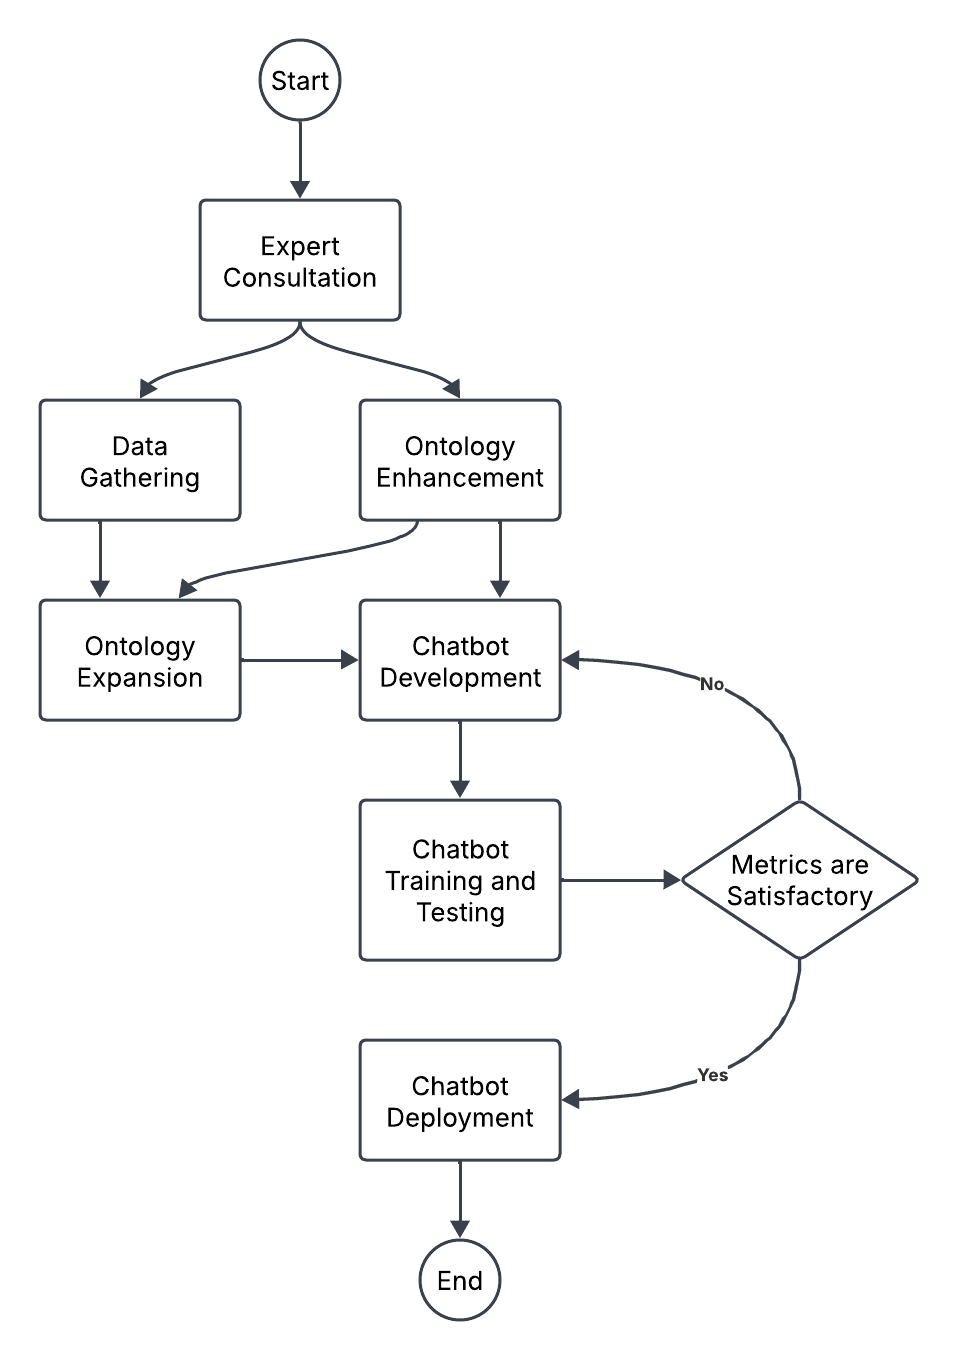
\includegraphics[width=0.8\linewidth]{figures/Process Diagram of Special Project.png}
    \caption{Process Diagram of Special Project}
    \label{fig:process diagram}
\end{figure}

\subsubsection{Data Collection} 
    The researchers will collect Panayanon myths, legends, and folktales from reliable resource persons. Other sources may be explored, including written records, research papers, and digital archives. For validation, the collected folk narratives will be presented and consulted on by the researchers with literature experts from the UPV Division of Humanities to verify the authenticity of the collected folk narratives. 
    
    The expected outcome of this process is a comprehensive and authentic collection of folk narratives that reflects the breadth and richness of Panayanon culture. This step is scheduled to start in December 2024 and must be accomplished halfway through January 2025, with a total duration of one and a half (1.5) months.
    
\subsubsection{Ontology Enhancement} 
    The researchers will engage in extensive consultations with experts from the UPV Division of Humanities. They will focus on creating new classes for the digital ontology,  specifically story elements such as geographical features and gender which are not present in the current ontology. Other possible classes may be explored. This will also be used to ensure consistency with standards in the field of literature.
    
    These new classes will be designed utilizing Protégé, an open-source ontology editor that supports OWL (Web Ontology Language) for formalizing domain knowledge. Each new class will be defined in terms of its relationships with other entities to create a structured and interconnected narrative representation. Protégé features such as logical constraints and reasoning will be utilized to ensure consistency and to infer relationships that enhance the semantic depth of the digital ontology.
    
    The expected outcome is an enhanced ontology structure that has more depth of information on Panayanon folk narratives than the original. This step is scheduled to start in mid-December 2024 and must be accomplished halfway through January 2025, with a total duration of one (1) month.

\subsubsection{Ontology Expansion}

    To follow good practices in the field of literature, the researchers will consult with experts to gain insights into the analysis of folk narratives, the identification of key story elements, and the contextual relationships between entities. With this, the researchers will closely read and examine each story from their collection, looking for relevant story elements and relationships. From their findings, they will expand the digital ontology by populating it with new stories, entities and relationships based on the enhanced ontological structure. 
    
    Protégé will be utilized for ontology expansion for its extensive support in OWL files and SPARQL querying, reasoning and consistency checking features, as well as collaboration features. Throughout this whole process, the researchers will present and consult with literature experts from the UPV Division of Humanities on the expanding ontology to validate the findings and ensure consistency with conventions and practices in the field of literature.
    
    The expected outcome is an expanded ontology that includes new details from the collected folk narratives based on the enhanced ontological structure. This step is scheduled to start in mid-January 2024 and must be accomplished by the end of April 2025, with a total duration of three and a half (3.5) months.

\subsubsection{Chatbot Development}
    In this step, the researchers will develop a chatbot prototype that can handle English queries from users, query the ontology to search for relevant data, and present the information to the user in comprehensible English sentences. Specifically, the researchers will utilize Python as the primary programming language to develop the chatbot, SpaCy as the natural language processing (NLP) library to analyze and process user queries, Rasa as the machine learning framework to extract the entities and intents of user inputs, GraphDB as the knowledge base to host the ontology, and a natural language generation (NLG) server to generate conversational responses to the user.
    
    Figure \ref{fig:rasa framework} shows the flow of data from user input to chatbot response generation. The ontology is converted into a graph database that can be queried for relevant information. The Rasa Agent works as a controller to easily orchestrate the dialogue flow of the chatbot, and manage the interaction of the different components. 
    
    When the user inputs a message, the NLU pipeline will first process it to extract its entities and intents. The extracted information is then passed through the Rasa Agent to the Dialogue Policies, which determine the appropriate action. If an external query is required, the Action Server requests information from the Knowledge Base. The data retrieved from the query is passed through an NLG server that contains RASA's contextual response rephrases to generate more natural, and conversational responses. The Rasa Agent receives this to then output the response to the user. The Tracker Store also receives the extracted entities, intents, and executed actions in order to maintain conversation history, which will help the Dialogue Policies make more context-aware decisions over time.

\begin{figure}[H]
    \centering
    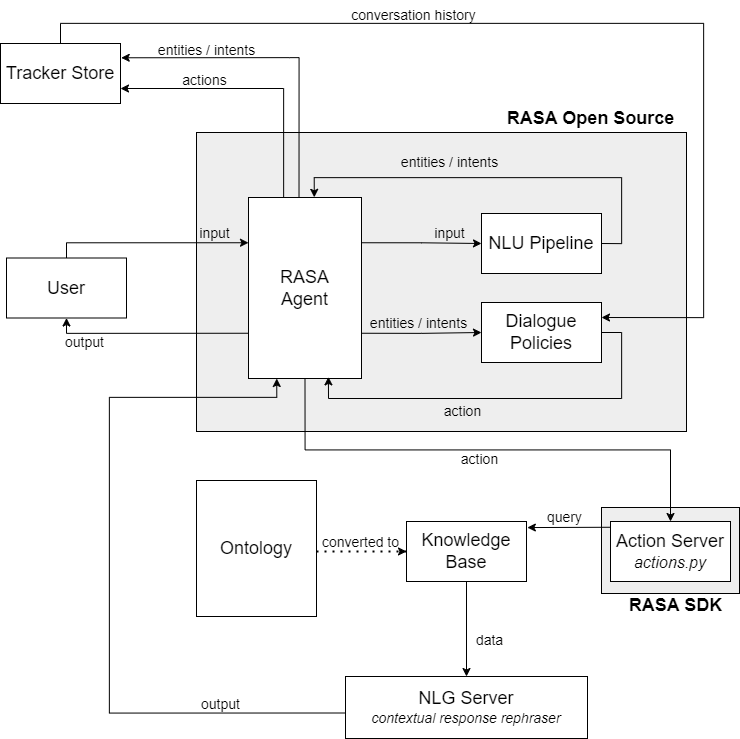
\includegraphics[width=\linewidth]{figures/Rasa Framework.png}
    \caption{Diagram of Rasa Framework}
    \label{fig:rasa framework}
\end{figure}

    Figure \ref{fig:nlu pipeline} illustrates RASA's natural language understanding pipeline. The first component, the spaCy tokeniser, splits the user's input into tokens. The second component, the spaCy featurizer, is a dense featurizer, that extracts features used for entity extraction, intent identification of the user's message, and response classification. The regex featurizer is a sparse featurizer, that creates a vector representation of the user's message using regular expressions for the purpose or entity extraction and intent identification. Next, is the lexical syntactic featurizer, a sparse featurizer, that creates lexical and syntactic features for a user's message for the purpose of entity extraction. The fifth component, count vectors featurizer, generates a bag-of-words representation of the bot user's message, intent, and response for the purpose of intent identification and response selection. The DIET Classifier, is a multi-task transformer architecture that is responsible for intent classification and entity extraction. The final component, is the Entity Synonym Mapper that maps entities to their synonyms if they appeared in the training data. The extracted entities and identified intents in the NLU pipeline, will then be passed to the dialogue policies of the chatbot to determine the appropriate actions that the bot will perform. 
    
    The components within the pipeline are used to process the user's input and extracts entities and intents from the user's input. This will be then queried through the knowledge base. Finally, the query results will be formatted into English through NLP techniques. With each iteration of the chatbot, the researchers will perform tests to verify chatbot query accuracy and response relevance, assess user interaction with the chatbot, and measure response times and optimize as needed.

\begin{figure}[H]
    \centering
    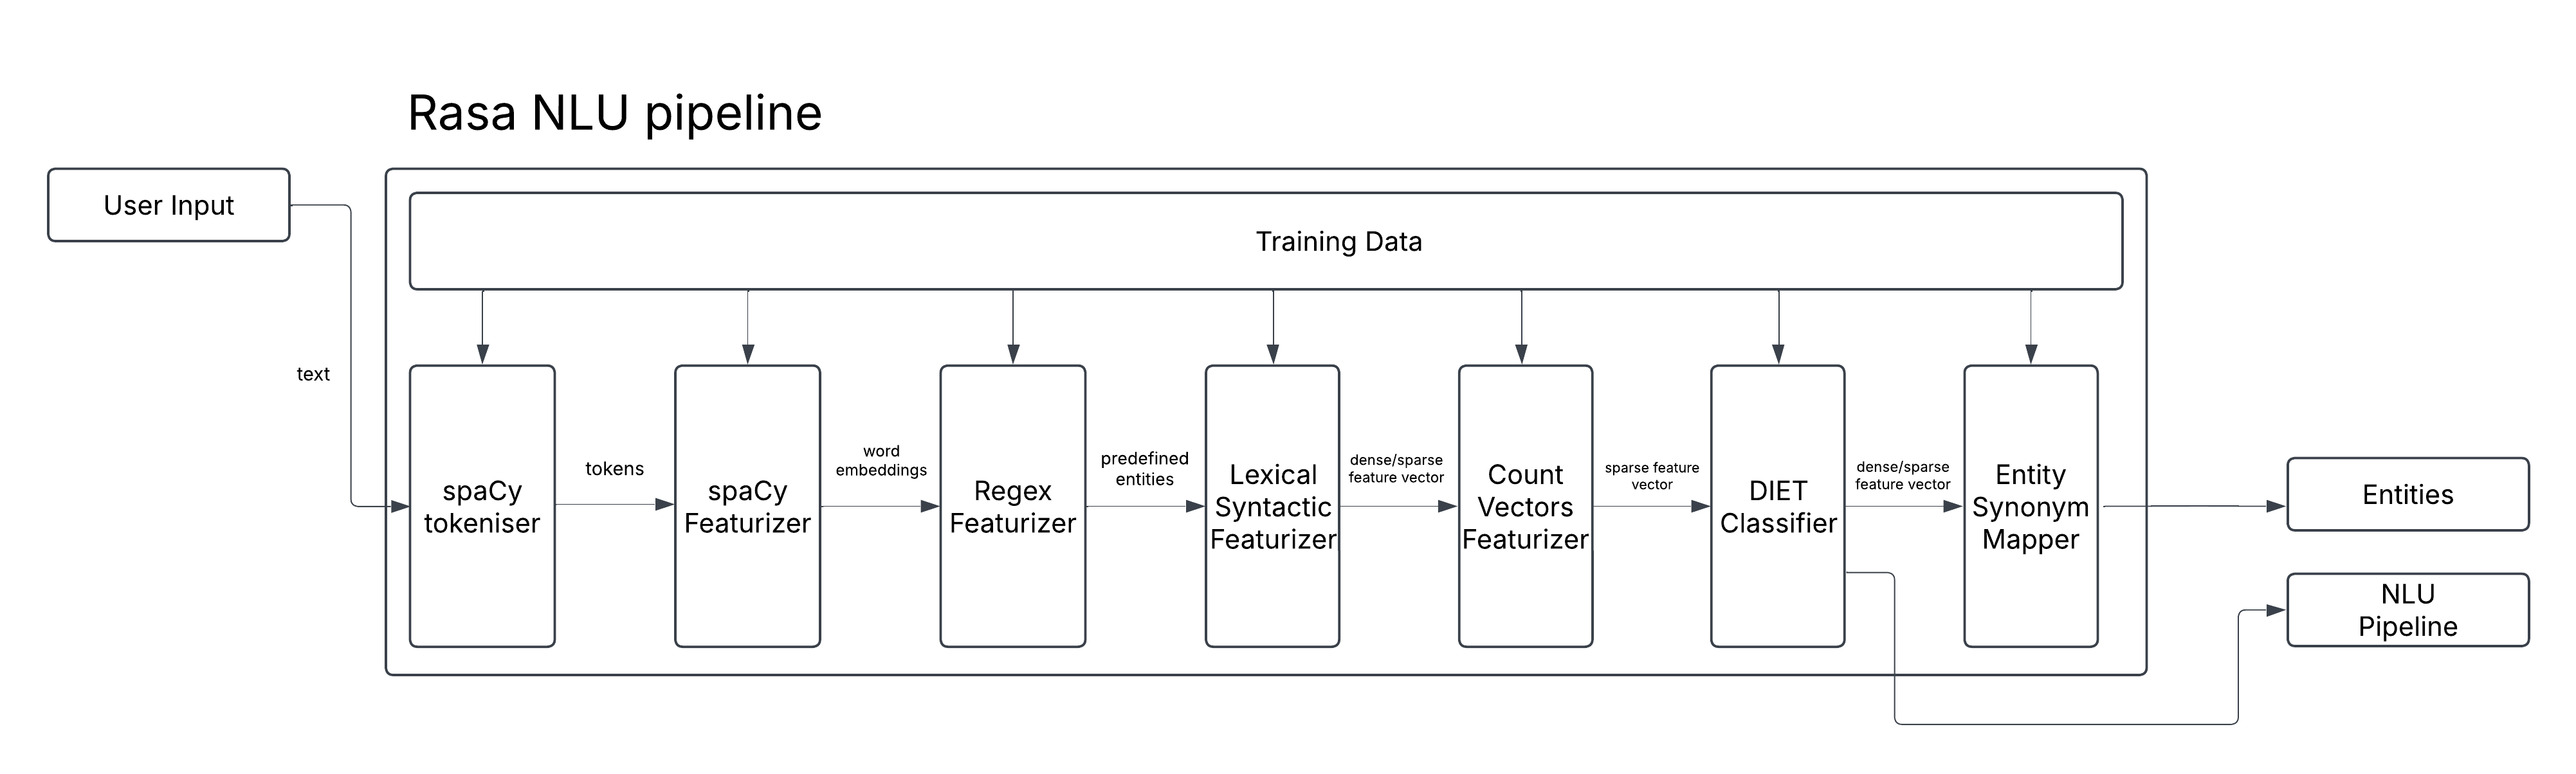
\includegraphics[width=\linewidth]{figures/NLU Pipeline.png}
    \caption{Diagram of NLU Pipeline}
    \label{fig:nlu pipeline}
\end{figure}

    The evaluation of the PAROT model by Ochieng (2020) involved the use of QALD-9 challenge metrics, including accuracy, recall, and F-measure. Similarly, the utilization of these metrics will be applied in the evaluation of the model under development of this special project. When the chatbot has achieved acceptable results in testing, it will then be deployed on a website.
    
    To enhance user experience, the chatbot will be designed to exhibit a conversational tone while maintaining the accuracy and professionalism required for ontology-based information retrieval. By incorporating NLG techniques, the chatbot will aim to engage users with dynamic and contextually appropriate responses that emulate human-like interaction. This conversational approach is expected to improve user engagement and satisfaction, especially when addressing more complex queries that may require clarification or follow-up interactions.

    With this chatbot, users will be able to interact with the ontology in natural language in a conversational and friendly manner. This is in pursuit of data querying, which is \citeA{manansala2007}) third and final pillar of ontology frameworks. The prototype chatbot will only serve to demonstrate the feasibility of chatbots as an information retrieval tool of the digital ontology.

    The expected output is a chatbot prototype that can semantically understand complex user questions in English, and answer them with accurate information from the ontology in a natural language format. This step is scheduled to start in February 2024 and must be accomplished by the end of May 2025, with a total duration of four (4) months.

\subsubsection{Documentation}

    The researchers will document relevant results and information throughout the project. It shall cover  data, methodology, results, and analysis. Additionally, insights and validations provided by expert consultations and testing phases will also be documented. Google Docs will be used for its simplicity and familiarity with the researchers, and Overleaf will be utilized for final formatting. 
    
    Applying software engineering principles, the researchers will also create diagrams such as use case diagrams, and sequence diagrams. For diagrams, computer assisted software engineering (CASE) tools will be utilized. The software will also be documented and stored in a GitHub repository.
    
    This step ensures that all information has been transparently communicated for future reference to be used by other researchers and interested parties. The expected output is complete project documents, including technical details, the software itself, and a final project report. This step is scheduled to start in December 2024 and must be accomplished by the end of May 2025, with a total duration of five (6) months.

\subsection{Calendar of Activities}

Table \ref{tab:timetableactivities} shows a Gantt chart of the activities.  Each bullet represents approximately
one week worth of activity.

%
%  the following commands will be used for filling up the bullets in the Gantt chart
%
\newcommand{\weekone}{\textbullet}
\newcommand{\weektwo}{\textbullet \textbullet}
\newcommand{\weekthree}{\textbullet \textbullet \textbullet}
\newcommand{\weekfour}{\textbullet \textbullet \textbullet \textbullet}

%
%  alternative to bullet is a star 
%
\begin{comment}
   \newcommand{\weekone}{$\star$}
   \newcommand{\weektwo}{$\star \star$}
   \newcommand{\weekthree}{$\star \star \star$}
   \newcommand{\weekfour}{$\star \star \star \star$ }
\end{comment}

\begin{table}[ht]   %t means place on top, replace with b if you want to place at the bottom
\centering
\caption{Timetable of Activities} \vspace{0.25em}
\begin{tabular}{|p{2in}|c|c|c|c|c|c|c|c|} \hline
\centering Activities (2025)            & Dec & Jan   & Feb & Mar & Apr & May \\ \hline
Data Collection                         & \weekfour  & \weektwo ~~~ &  &  &  & \\ \hline
Ontology Enhancement                    & ~~~\weektwo  & \weektwo ~~~ & & & & \\ \hline
Ontology Expansion                      & & ~~~\weektwo & \weekfour & \weekfour & \weekfour & \\ \hline
Chatbot Development                     & & & \weekfour & \weekfour & \weekfour & \weekfour \\ \hline
Documentation                           & \weekfour  & \weekfour & \weekfour & \weekfour & \weekfour & \weekfour \\ \hline


\end{tabular}
\label{tab:timetableactivities}
\end{table}

